\section{Asinchroninės (angl. “asynchronous”) integracijos}

\subsection{Asinchroninių integracijų principas}
Asinchroninės integracijos yra vis labiau populiarėjančios ir vis dažniau sutinkamos informacinėse sistemose.
Tokio tipo komunikavimas yra labai tinkamas ilgiems procesams ir daug žingsnių turinčioms operacijoms \cite{Bk2}.
Pačio integracijos tipo principą galima būtų apibūdinti dviem žodžiais: „nelaukianti atsakymo“. Prisimenant jau
aptartą serverio ir kliento modelį, sinchroninių integracijų metu klientas siunčia užklausą ir laukia atsakymo iš serverio.
Asinchroninių integracijų metu, klientas siunčia užklausa ir priklausomai nuo naudojamos technologijos serveris gali grąžinti
arba paprastą atsakymą, kad užregistravo užklausą, arba išvis nieko nepranešti. Tokiu būdu klientas dar negauna resurso, kurio jam reikia
ir neblokuojamas gali vykdyti kitus procesus arba siųsti kitas užklausas. Serveris tuo metu užregistraves užklausą, bando gauti klientui reikiamą
resursą arba vykdyti užklausoje nurodytą veiksmą. Klientas tik po kurio laiko vėl siunčia užklausą serveriui, tik šįkart jau neprašydamas resurso
ir neliepdamas įvykdyti veiksmų, bet klausdamas ar galima pasiimti resursą, ar jau įvykdytas veiksmas ar jų seka.
Serveris užklaustas kliento, jeigu yra įvykdęs savo užduotį, grąžina klientui atsakymą su užklaustu resursu. Kitu atveju klientui iš serverio
gauna atsakymą, kad pradėtas procesas dar yra neužbaigtas. Šį veikimo principą vaizduoja pateikta schema (\ref{img:asynchronous-communication} pav.)

\begin{figure}[H]
  \centering
  \includegraphics[scale=0.45]{img/asynchronous-communication}
  \caption{Asinchroninio komunikavimo schema.}
  \label{img:asynchronous-communication}
\end{figure}
\break

Toks yra tradicinis asynchroninio komunikavimo principas. Kuriant mikroservisų architektūra paremtą informacinę sistemą,
neretai susiduriama su tokiu atveju, kai norint sukurti resursą arba įgyvendinti procesą neužtenka tik dviejų servisų įsikišimo.
Tokiais atvejais pasinaudojant asinchroninėmis integracijų technologijomis, galima perduoti žinutę ne vienam servisui, o keliems iš karto.
Tada keli servisai gali klausytis šių žinučių ir į jas reaguoti vienu metu vykdant savo atsakomybes. Visiem servisams baigus darbą,
jie taip pat sukuria žinutes apie savo darbo pabaigą tik, kai visos žinutės yra išsiųstos, būna galutinai sukuriamas resursas arba procesas
tampa įvykdytu. Įgyvendti tokius procesus nebūna paprasta ir dažnu atveju reikalingos papildomos technologijos įgyvendinimui.
Taip pat turi būti servisas atsakingas už tikrinimą ar visi savo procesus atliekantys servisai baigė darbą. Šis servisas turi
saugoti proceso būsena (angl. \textit{„state“}) realiu laiku. Ši būsena procesus vykdantiems servisams turėtų būti nežinoma.
Toks pavyzdys yra vadinamas „publikavimo/prenumeravimo“ (angl. \textit{„publish/subscribe“}) mechanizmu. Šiame mechanizme yra
servisai, kurie prenumeruojasi prie žinučių apie naujo resurso sukūrimo inicijavimą ir patys paskelbia pranešimus apie savo procesų pabaigą.
Servisas, kuris saugo proceso būseną, prenumeruojasi prie šių pranešimų ir atnaujiną būseną. Toks modelis yra aprašomas Espen Johnses magistriniame darbe
„Reliable Asynchronous Communication in Distributed Systems“ \cite{MstrThs1}. Taip pat šis mechanizmas yra labai plačiai naudojamas
įvykiais paremtose (angl. \textit{„event-based“}) architektūrose.

Verta paminėti, kad toks komunikavimo tipas yra neblokuojantis (angl. \textit{„non-blocking“}). Tai reiškia, kad skirtingai nei sinchroninių
komunikacijų metu, servisas išsiuntęs užklausą, gali toliau vykdyti kitus procesus. Vienas iš pavyzdžių būtų bekuriant naują resursą leisti
vartotojui modifikuoti kitus nesusijusius resursus.

Siekant geriau išaiškinti, kaip veikia asinchroninis komunikavimas mikroservisų sistemose, išanalizuosime modelinė situacija, kur komunikavimas vyktų būtent
minėtu būdu. Patį sistemos modelį pasirinksime tokį patį, koks buvo naudojamas apibūdinti sichroninį komunikavimą.
Taigi, asinchroniniu komunikavimo modeliu servisas atsakingas už studentų duomenų tvarkymą bus informuotas apie naujo studento kūrimo inicijavimą.
Šis servisas savo duomenų bazėje sukuria naują įrašą ir vykdo tokius veiksmus eilės tvarka:

\begin{enumerate}
  \item Studentų duomenų servise sukuriama žinutė apie studento užregistravimo incijavimą.
  \item Dokumentų servisas prenumaruojasi tokią žinutę ir ją gavęs, sugeneruoją dokumentą ir sukuria žinutę apie
   sėkmingą sugeneravimą. Nesekmės atveju sukuria žinutę kad nepavyko sukurti tokio dokumento.
  \item Tvarkaraščių servisas taip pat prenumeruojasi prie inicijavimo žinutės ir tokią gavęs sugeneruoja tvarkaraštį studentui.
  Sėkmingai įvykdęs darbą, kaip ir dokumentų servisas, sukuria žinutę apie sėkmingą sugeneravimą, o nesėkmės atveju žinutę, kad nepavyko užbaigti proceso
  arba jis užbaigtas nekorektiškai.
  \item Elektroninių laiškų servisas irgi prenumeruojasi inicijavimo žinutę ir ją gavęs vykdo savo atsakomybes - išsiųsti laiškus dėstytojams.
  Procesui pasibaigus, sėkmingai ar ne, išsiunčiama žinutė apie proceso pabaigos rezulatatus.
  \item Studentų servisas prenumeruojasi prie visų žinučių, kurias siunčia su studento kūrimu susiję servisai. Gaudamas šiuos pranešimus, servisas pas save išsisaugo
  esama kuriamo studento situaciją. Jeigu buvo gautas pranešimas apie nesėkmingą kažkurio iš tarpinių procesų darbą, tada servisas pasižymi, kad tokio studento sukurti nepavyko.
  Kitu atveju, jeigu viskas įvyko sėkmingai, tai servisas patvirtina sėkmingą studento užregistravimą ir baigią procesą. 
\end{enumerate}

Asinchorninio komunikavimo metu, visi procesai žinutes gauna neptertraukdami vienas kito. 
Tokią veiksmų seką vaizdžiai parodo tokia ši schema (\ref{img:asynchronous-microservice-model} pav.):

\begin{figure}[H]
  \centering
  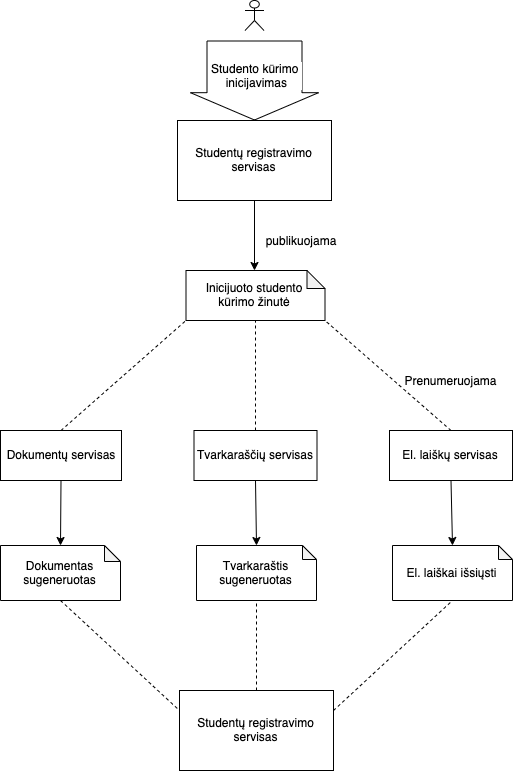
\includegraphics[scale=0.6]{img/asynchronous-microservice-model}
  \caption{Asinchroninio komunikavimo mikroservisuose schema.}
  \label{img:asynchronous-microservice-model}
\end{figure}

Toks modelis yra tik vienas iš būdų kokiu principu gali būti realizuojamas asinchroninis komunikavimas.

\subsection{Asinchroninių integracijų technologijos}
Yra daug skirtingų būdų ir technologinių, siekiant įgyvendinti asinchronines integracijas tarp mikroservisų.
Kai kurios kalbos jau yra pritaikytos asinchroninėms integracijoms. Pavyzdžiui JAVA nuo 8 versijos savo aplikacijų programavimo sąsajoje
jau pristatė „Completable Future“ modelį, kuriame pagalbinių metodų ir klasių  pagalba galima įgyvendinti asinchroninius komunikavimus.
Remiantis Vineet John ir Xia Liu publikacija „Apklausa apie paskirstytas pranešimų brokerius“ (angl. \textit{„A Survey of Distributed Message Broker Queues“}) \cite{Sur1}
pranešimų brokeriai (angl. \textit{„Message Brokers“}) yra populiaurias komunikavimo pasirinkimas paskirstytose sistemose. Bendravimas per pranešimų brokerius
iš savo principo yra asinchroninis. Dėl pranešimų brokerių populiarimo, kaip technologini tipą šiame darbe aptarsime būtent šią technologiją.

Dar 2019 metų gale publikuotame leidinyje apie modernius pranešimų brokerius \cite{Misc8} lyginamos 3 labai populiarūs 
pranešimų brokeriai:

\begin{enumerate}
  \item Apache Kafka.
  \item Rabbit MQ
  \item NATS.
\end{enumerate}

Šios trys technologijos yra gan panašios savo principais, bet renkantis, kurią iš jų naudoti kuriant sistemą reikia
gerai atsižvelgti į jų privalumus ir trūkumus. Kaip ir minima PHilippe Dobbelaere ir Kyums Sheykh Esmaili publikuotame straipsnyje „Kafka prie RabbitMQ“
(anlg. \textit{„Kafka versus RabbitMQ“}) \cite{Misc4}, nėra geresnio ar blogesnio iš šių dviejų pranešimų brokerių. Abu brokeriai buvo sukurti siekiant 
išspręsti skirtingas problemas ir įgyvendinti skirtingus tikslus. Neišimtis yra ir su NATS. Nor visi brokeriai veikia panašiu mechanizmu, skirtingiem prioritetams 
reikia skirtingų brokerių.

Šie pranešimų brokeriai, veikia pagal „publikavimo/prenumeravimo“ mechanizmą, kuriame „publikuotojai“ siunčia pranešimus
į brokerį, o „prenumeratoriai“ skaito pranešimus. Į brokerį atsiunčiami pranešimai būna saugomi eilėje, iš kurios 
„prenumeratoriai“ skaito prenumeruotas žinutes.





